\documentclass[a4paper]{article}
\usepackage[utf8]{inputenc}
\usepackage[italian]{babel}
\usepackage{csquotes}
\usepackage{hyperref}
\usepackage{graphicx}
\usepackage{float}
\usepackage{listings}
\usepackage{xcolor}
\usepackage[style=alphabetic]{biblatex}
\bibliography{bibliography.bib}

\definecolor{backcolour}{rgb}{0.95,0.95,0.92}
\lstdefinestyle{mystyle}{
    backgroundcolor=\color{backcolour},   
    basicstyle=\ttfamily\footnotesize,
    breakatwhitespace=false,         
    breaklines=true,                 
    captionpos=b,                    
    keepspaces=true,                                   
    showspaces=false,                
    showstringspaces=false,
    showtabs=false,                  
    tabsize=2
}

\lstset{style=mystyle}

\begin{document}
\section*{Abstract}
Una sfida fondamentale per gli standard che trattano dati sanitari è come gestire la grande variabilità causata dai diversi tipi di processi e prodotti.
Durante lo scorrere del tempo poi, molti campi e opzioni possono essere aggiunte alla specifica, causando gradualmente costi e complessità aggiuntive alla
implementazione da produrre. L'alternativa è crearsi estensioni dedicate, ma anche questa comporta molti problemi di implementazione.
Anche i registri sanitari stanno diventando sempre più digitalizzati. Quando i pazienti utilizzano sistemi appartenenti al sistema sanitario, le loro cartelle cliniche
elettroniche (i loro dati medici) devono essere disponibili, rilevabili e comprensibili. Inoltre, per supportare il supporto di decisioni cliniche automatizzate e altre elaborazioni
basate su macchine, i dati devono anche essere strutturati e standardizzati.
Questo progetto di tesi ha approfondito un ambito di questo problema, la gestione di dati sanitari provenienti da dispositivi indossabili, attraverso lo sviluppo di un progetto java
che simula la creazione di dati da parte di dispositivi medici e li converte nello standard FHIR, diffuso in tutto il mondo e su cui si basa anche il fascicolo sanitario della regione Lombardia. 


\clearpage
\null
\thispagestyle{empty}

\clearpage

\tableofcontents
\newpage
\section{Introduzione}
\subsection{Scopo}
Oggetti come smartwatch, fasce cardio, bilance e termometri cosiddetti "intelligenti" stanno prendendo sempre più piede nelle vite della gente comune.
Come altri prodotti di consumo però esistono ovviamente diversi produttori sul mercato ed ognuno sviluppa il proprio protocollo ed applicativo dedicati
per gestire la comunicazione e la visualizzazione dei dati sanitari.
Questa tendenza rischia di non sfruttare le potenzialità in ambito sanitario che questi rilevatori di parametri vitali offrono, poiché potrebbero essere
utili in futuro grazie allo sviluppo della \textbf{telemedicina}.
Facciamo un esempio: una persona con una malattia cronica, come ad esempio il diabete, utilizza un rilevatore smart per tenere la glicemia sotto controllo.
I dati prodotti sono visualizzabili nell'applicazione del prodotto, risultando così "confinati".
Attraverso un sistema unico invece, si potrebbe utilizzare il dispositivo che riceve ed elabora i dati (cellulare personale, pc) come gateway, cioè come intermediario tra tutti i dispositivi
medici indossabili e un sistema remoto di storage ed elaborazione di dati sanitari, come il fascicolo sanitario.
In questo modo, la grande quantità di dati potrebbe essere analizzata in caso di bisogno dal personale medico, contribuendo a tracciare un quadro completo dello stato di salute dei pazienti.
\subsection{Obiettivi}
Sviluppo di un progetto Java che simula la creazione di dati da parte di dispositivi medici (osservazioni) seguendo le direttive dello standard ISO/IEEE 11073-10206 - ACOM e li converte nello
standard FHIR allo scopo di favorire l'interoperabilità tra sistemi differenti.
Dovrà quindi essere sviluppato un convertitore da ACOM a FHIR, prendendo in esame alcuni dispositivi specifici e le osservazioni che possono generare. 
\section{Background}
\subsection{ISO/IEEE 11073-10206 - ACOM}
\subsubsection{Ambito e finalità}
Questo standard definisce un modello di contenuto astratto (ACOM: Abstract Content Information Model) per i dispositivi di salute personale.
L'obiettivo di IEEE 11073-10206 è quello di documentare le informazioni in un Personal Health Device, da qui in poi chiamato PHD e il contenuto delle osservazioni sanitarie che vengono inviati dal PHD in modo che quando un'osservazione viene ricevuta dal PHD, indipendentemente dal protocollo utilizzato per eseguire
la comunicazione, le informazioni sanitarie sono \textbf{complete}, \textbf{coerenti} e \textbf{inequivocabili}.
IEEE 11073-10206 definisce un modello informativo astratto ed object-oriented allo scopo di rappresentare un PHD e le osservazioni che può generare.
Specifica quali informazioni devono essere presenti e le relazioni tra elementi informativi nel modello. Modella le osservazioni in modo generico
concentrandosi sulle informazioni contenuto nella presentazione delle misure sanitarie.
La figura~\ref{fig:overallContextOfWork} mostra le categorie e i tipi tipici di dispositivi nell'ambito della salute personale. I PHD (ad esempio: monitor della pressione sanguigna, bilance e pedometri) raccolgono informazioni su una o più persone, trasferendole poi ad un PHG, Personal Health Gateway (ad esempio: telefono cellulare, apparecchio sanitario o pc) per la raccolta, la visualizzazione e l'eventuale trasmissione successiva. Il PHG può anche trasmettere i dati a servizi di supporto remoto per ulteriori analisi o per permettere la gestione delle malattie.

\begin{figure}[H]
    \centering
    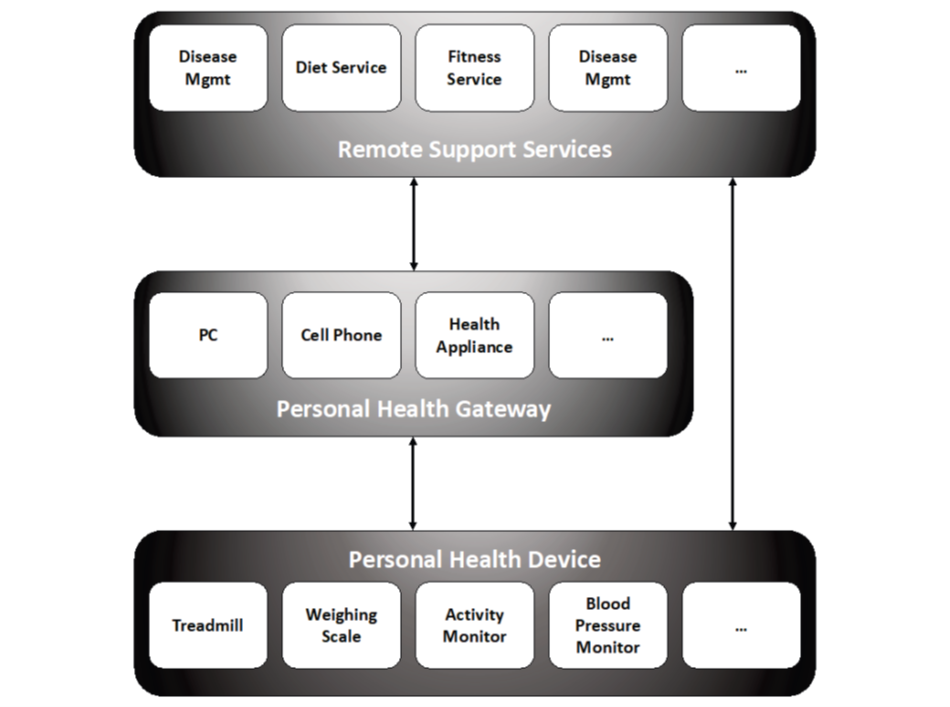
\includegraphics[width=1\textwidth]{figures/overall context of work.png}
    \caption{Contesto di ACOM}
    \label{fig:overallContextOfWork}
\end{figure}

\subsubsection{Classe Osservazione}
La classe di osservazione ACOM fornisce un modello generico per esprimere osservazioni da dispositivi di salute personale.
E' basata sull'oggetto metrico descritto dallo standard ISO/IEEE 11073-20601 e condivide molti attributi della risorsa analoga osservazione presente nello standard HL7 FHIR.
Come si può vedere in figura \ref{fig:observationClass}, la classe si compone di una serie di elementi concettuali, tutti derivanti dall'oggetto \textbf{Observation}.

\begin{figure}[H]
    \centering
    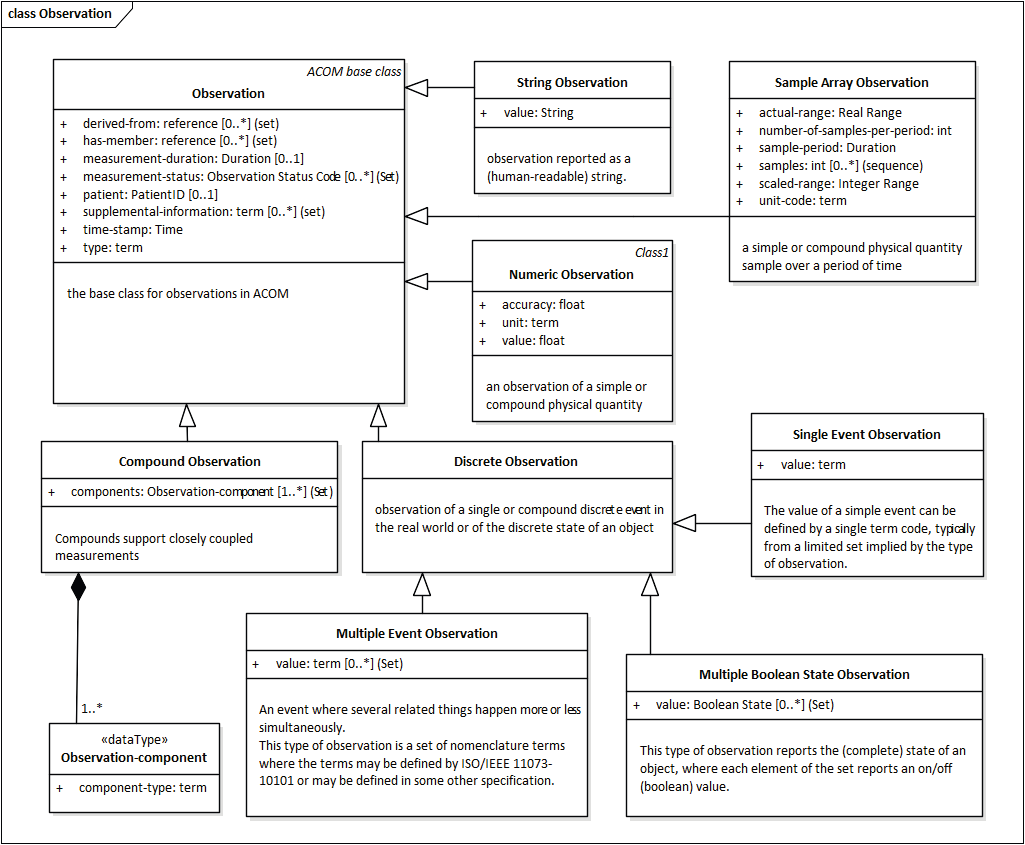
\includegraphics[width=1\textwidth]{figures/observation class.png}
    \caption{Classe Observation}
    \label{fig:observationClass}
\end{figure}

\subsubsection{Specializzazioni su dispositivi}
Le specializzazioni dei dispositivi sono usate in questo standard per definire il contenuto informativo di uno specifico tipo di PHD.
Sono classi che modellano alcuni tipi di PHD particolari (appartenenti alla classe IEEE 11073-104XX), di conseguenza contengono al loro interno le informazioni basilari sulla struttura del PHD: \textbf{Power} rappresenta il tipo di alimentazione e le operazioni che mantengono in attività il PHD; \textbf{Clock}  e \textbf{SystemInfo},
un oggetto che modella il PHD e un oggetto Observation che modella le osservazioni.


\begin{figure}[H]
    \centering
    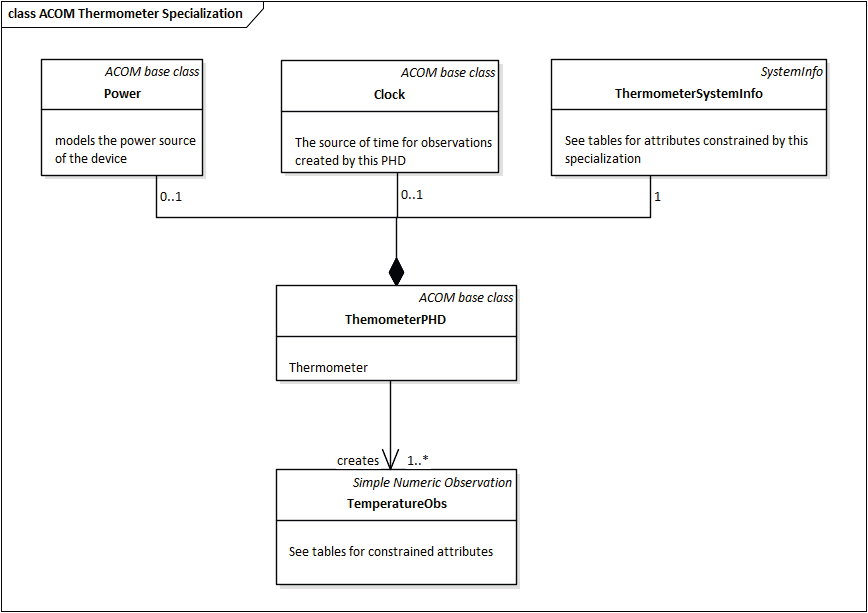
\includegraphics[width=1\textwidth]{figures/ACOM thermometer specialization class.png}
    \caption{classe ACOM che modella il dispositivo Termometro}
\end{figure}

\subsection{FHIR}
\textbf{FHIR}, Fast Healthcare Interoperability Resources, è uno standard di interoperabilità sanitaria di HL7 (associazione non profit internazionale che si occupa di gestire standard per la sanità)
che consente a una moltitudine di sistemi di scambiare informazioni sanitarie utilizzando modelli di dati concordati. In FHIR, questi modelli di dati sono semplici, diretti, contemporaneamente
leggibili da uomo e computer e, quando combinati, abbastanza robusti da trasmettere informazioni sanitarie complesse.
Gli obbiettivi primari di FHIR sono:
\begin{itemize}
    \item creare uno standard da utilizzare tra diverse piattaforme informatiche che si occupano di dati sanitari
    \item rendere l'interoperabilità in tempo reale più semplice
\end{itemize}
In definitiva, FHIR riduce la curva d'apprendimento, rende l'interoperabilità più semplice e permette di creare in modo più veloce e semplice applicativi.

\subsubsection{Struttura}
Il componente base dello standard FHIR è la struttura chiamata \textbf{risorsa}. Tutti gli oggetti FHIR che possono essere inviati sono definiti come risorsa.
La filosofia su cui si basa FHIR è costruire un set base di risorse che, sia da sole sia combinate, possano soddisfare la maggioranza dei casi d'uso esistenti.
La modellazione FHIR usa un approccio compositivo, cioè implementa i casi d'uso combinando insieme più risorse singole.

\subsubsection*{Risorse}
In FHIR, i dati sanitari sono divisi in categorie, come ad esempio pazienti, risultati di laboratorio ed osservazioni.
Ciascuna di queste categorie è descritta approfonditamente all'interno di una risorsa FHIR, che include i suoi dati, la terminologia e altre regole che insieme formano un elemento scambiabile.
Tutte le risorse hanno le seguenti features in comune:
\begin{itemize}
    \item un identificatore per la risorsa, tipicamente un URL che specifica dove si trova la risorsa
    \item metadati comuni
    \item un sommario in formato XHTML, facilmente leggibile
    \item un insieme di data elements, diversi per ogni tipo di risorsa
    \item un framework che permette l'estensibilità, in grado di supportare variazioni della struttura
\end{itemize}

Le istanze delle risorse possono essere rappresentate in diversi formati quali XML, JSON o RDF e attualmente esistono 157 differenti tipi di risorsa nella specifica FHIR.

\subsubsection*{Profili delle risorse}
La specifica base di FHIR descrive un insieme di risorse di base, framework e API che vengono utilizzati in diversi contesti nel settore sanitario. Tuttavia, esiste una notevole variabilità nella gestione dei sistemi sanitari, sia tra diversi stati, sia all'interno dello stesso sistema; infatti devono rispondere a diverse normative, con requisiti e pratiche richieste spesso molto differenti.
Per questo motivo, la specifica FHIR è una "specifica di piattaforma" - crea una piattaforma comune o una base su cui vengono implementate diverse soluzioni. Di conseguenza, questa specifica richiede solitamente ulteriori adattamenti ai particolari contesti di utilizzo. Tipicamente, questi adattamenti specificano:
\begin{itemize}
    \item Regole riguardo gli elementi delle risorse che vengono utilizzati e quali elementi vengono aggiunti che non fanno parte della specifica di base
    \item Regole su quali funzionalità delle API vengono utilizzate e la loro implementazione
    \item Regole su quali terminologie vengono utilizzate in particolari elementi
    \item Descrizioni di come gli elementi delle risorse e le funzionalità delle API si  relazionano ai requisiti e implementazioni locali
\end{itemize}
In particolare, i \textbf{profili} sono un insieme di vincoli su una risorsa utili a definire la sua struttura.
Vengono essenzialmente utilizzati in due modi:
\textbf{Resource profiles} descritti utilizzando l'elemento \textit{CapabilityStatement.rest.resource.profile};
\textbf{Supported profiles} descritti utilizzando l'elemento \textit{CapabilityStatement.rest resource.supportedProfile}.
\subsubsection*{CapabilityStatement.rest.resource.profile}
Questi profili descrivono le caratteristiche generali supportate dal sistema per ogni tipo di risorsa.
Tipicamente, questo è il superset di tutti i diversi casi d'uso implementati dal sistema.
\subsubsection*{CapabilityStatement.rest.resource.supportedProfile}
Questi profili descrivono le informazioni prodotte e gestite dal sistema in base a ciascun caso d'uso. Alcuni esempi di utilizzo per questi tipi di profili sono:
\begin{itemize}
    \item Un servizio di laboratorio che produce una serie di diversi rapporti - chimica generale, emocromo, ecc. La maggior parte dei laboratori possono generare anche centinaia di rapporti diversi
    \item Un gestore delle cure che gestisce un insieme di diversi tipi di piani di cura e risorse cliniche associate.
\end{itemize}
Questi profili rappresentano diversi casi d'uso che portano a gestire le risorse del tipo indicato dal CapabilityStatement.rest.resource.type in modo diverso.
Affinché un sistema produttore e un sistema consumatore possano scambiare dati con successo basandosi su uno di questi profili supportati, non è sufficiente sapere che i sistemi hanno profili che si sovrappongono per il caso d'uso di interesse; il consumatore deve essere in grado di filtrare l'insieme totale delle risorse messe a disposizione dal sistema produttore e gestire solo quelle rilevanti per il caso d'uso.
Se consideriamo un sistema di laboratorio che genera migliaia di rapporti al giorno, circa l'1\%  di questi rapporti è un particolare rapporto endocrinologico che un sistema di supporto decisionale sa come elaborare. Entrambi i sistemi dichiarano di supportare il particolare profilo del rapporto endocrinologico, ma come fa il sistema di supporto decisionale a trovare effettivamente i rapporti endocrinologici che sa come elaborare?
Una possibile opzione prevede che il sistema di supporto decisionale riceva ogni singolo rapporto proveniente dal sistema di laboratorio, verifichi la conformità al profilo e successivamente decida se procedere con l'elaborazione. Verificare se una risorsa è conforme a un particolare profilo è un'operazione semplice, ma molto inefficiente in quanto il sistema di supporto decisionale deve ricevere ed elaborare 100 volte pi`u risorse di quante ne utilizzi effettivamente.
Per aiutare un consumatore a trovare l'insieme corretto di rapporti per un caso d'uso, un produttore di risorse può:
\begin{itemize}
    \item dichiarare con asserzioni di profilo documentando i profili a cui sono conformi (questo consente l'indicizzazione per profilo)
    \item cercare i profili dichiarati tramite il parametro di ricerca "profile", se il parametro di ricerca è supportato.
\end{itemize}

\subsubsection*{Esempio istanza di una risorsa}
Di seguito è fornito un esempio di come un paziente viene rappresentato tramite un oggetto FHIR in formato JSON.
E' possibile notare la presenza delle features descritte in precedenza.
\begin{figure}[H]
    \centering
    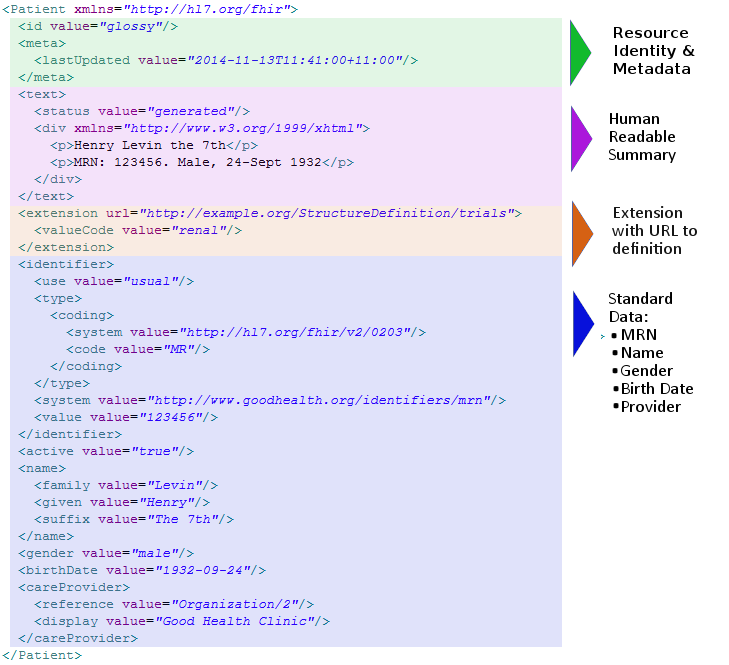
\includegraphics[width=1 \textwidth]{figures/esempio paziente.png}
    \label{fig:esempioPaziente}
\end{figure}
\subsubsection{Risorsa Osservazione}
Le osservazioni sono un elemento fondamentale nel mondo sanitario, utili per supportare diagnosi di malattie, monitare progressi
dovuti a cure mediche o determinare pattern ricorrenti nella popolazione.
La maggioranza delle osservazioni possono essere rappresentate da coppie nome-valore coadiuvate da metadati, ma esistono anche tipi di osservazioni con strutture più complesse.
Gli usi della risorsa Osservazione sono molteplici:
\begin{itemize}
    \item Parametri vitali come pressione sanguigna, temperatura corporea o battito cardiaco
    \item Dati di laboratorio derivati da esami medici, come la quantità di glucosio nel sangue
    \item Dati risultanti dallo studio di immagini mediche, come la densità ossea o la misurazione fetale
    \item Sintomatologie cliniche
    \item Misurazioni di macchinari specifici, come elettrocardiogramma o pulsossimetro
    \item Impostazioni di macchinari
    \item Caratteristiche fisiche personali, come ad esempio il colore dei capelli o degli occhi
    \item Storia medica familiare: malattie croniche famigliari, parenti fumatori, etc.
\end{itemize}
Tipicamente, un'osservazione riguarda il soggetto - un paziente, un gruppo di pazienti, una località o un dispositivo - e la distinzione tra il soggetto e ciò che è direttamente
misurato per un'osservazione è specificata nel codice dell'osservazione stessa (ad esempio, "Glucosio nel sangue") e non necessita di essere rappresentata separatamente.
Tuttavia, tre attributi possono essere utilizzati per rappresentare il focus dell'osservazione se non è il soggetto stesso.
\subsubsection*{Profilare un'osservazione}
Nella sua forma più semplice, un'istanza di risorsa può consistere solo di un codice, un valore e un flag di stato.
La rilevanza di altre proprietà varierà in base al tipo di osservazione.
I profili sono creati per fornire linee guida sulla cattura di determinati tipi di osservazioni per un determinato caso d'uso.
La risorsa Osservazione si concentra sul livello di dettaglio catturato dalla maggior parte dei sistemi.
Tuttavia, per un dato caso d'uso, potrebbero esserci vincoli aggiuntivi e informazioni supplementari rilevanti in determinate circostanze.
Come per altre risorse, le estensioni possono essere utilizzate per introdurre questa complessità aggiuntiva.
Il profilo \textbf{FHIR Vital Signs} stabilisce le aspettative minime per la risorsa Osservazione per registrare, cercare e recuperare i segni vitali associati a un paziente, che includono i segni vitali primari oltre a misurazioni aggiuntive come altezza, peso e BMI (Body Mass Index).
Quando un'implementazione FHIR supporta uno qualsiasi dei segni vitali elencati di seguito, l'implementazione dovrà conformarsi a questo profilo per l'osservazione dei parametri vitali.
Un'osservazione che rispetta il profilo appena descritto deve quindi avere:
\begin{itemize}
    \item uno status
    \item un codice appartenente alla categoria "vital signs"
    \item un "valore magico", che descrive cosa l'osservazione sta misurando.
          A tal proposito è necessario specificare che lo standard scelto è \textbf{LOINC} per la sua diffusione capillare
    \item un paziente
    \item una data che indica quando l'osservazione è stata rilevata
    \item un valore numerico e un'unità di misura facente parte dello standard \textbf{UCUM} (Unified Code for Units of Measure)
\end{itemize}
Approfondendo il formato dei valori, è importante specificare che quando un valore di risultato è rappresentato come un concetto predefinito utilizzando un codice, viene utilizzato il datatype valueCodeableConcept.
Questo elemento è vincolato a un set di valori composto da una nomenclatura standard come SNOMED CT o da valori di risultato codificati di un sistema sorgente ("locale").
I risultati possono essere codificati in più set di valori basati su diversi sistemi di codici e questi possono essere mappati utilizzando la risorsa ConceptMap e/o forniti come codifiche aggiuntive direttamente nell'elemento, come mostrato nell'esempio seguente.
\begin{lstlisting}
            "valueCodeableConcept": {
                "coding": [
                    {
                        "system": "http://snomed.info/sct",
                        "code": "260385009",
                        "display": "Negative"
                    }, {
                        "system": "https://acme.lab/resultcodes",
                        "code": "NEG",
                        "display": "Negative"
                    }
                ],
                "text": "Negative for Chlamydia Trachomatis rRNA"
            }
        \end{lstlisting}
\subsubsection{Esempio osservazione FHIR}
\begin{lstlisting}
    {
        "resourceType": "Observation",
        "id": "body-temperature",
        "meta": {
            "profile": [
                "http://hl7.org/fhir/StructureDefinition/vitalsigns"
            ]
        },
        "text": {
            "status": "generated",
            "div": "<div xmlns=\"http://www.w3.org/1999/xhtml\"><p><b>Generated Narrative: Observation</b><a name=\"body-temperature\">"
        },
        "status": "final",
        "category": [
            {
                "coding": [
                    {
                        "system": "http://terminology.hl7.org/CodeSystem/observation-category",
                        "code": "vital-signs",
                        "display": "Vital Signs",
                        "userSelected": false
                    }
                ],
                "text": "Vital Signs"
            }
        ],
        "code": {
            "coding": [
                {
                    "system": "http://loinc.org",
                    "code": "8310-5",
                    "display": "Body temperature",
                    "userSelected": false
                }
            ],
            "text": "Body temperature"
        },
        "subject": {
            "reference": "Patient/example"
        },
        "encounter": {
            "reference": "Encounter/example"
        },
        "effectiveDateTime": "2024-05-24T10:27:02Z",
        "valueQuantity": {
            "value": 36.5,
            "unit": "C",
            "system": "http://unitsofmeasure.org",
            "code": "Cel"
        }
    }  

\end{lstlisting}
\section{Sviluppo}
Il progetto svolto si può essenzialmente dividere in tre parti: implementazione di classi che modellano osservazioni ACOM,
classe che modella osservazione FHIR ed un convertitore 
\section{Conclusione}
Questo progetto di tesi presenta una prima versione dello sviluppo di un convertitore universale da ACOM a FHIR.
Tuttavia, come presentato, esistono molti altre osservazioni generate da dispositivi medici da modellare.
Sarebbe quindi utile approfondire il progetto modellando come specificato dallo standard ACOM anche i dispositivi medici,
così da ottenere una simulazione realistica della realtà.
\printbibliography
\end{document}